\section{相关工作}

\cpar{大型多模态模型。} 长期以来的研究目标之一是开发能够通过多种模态感知世界的模型,类似于人类的感官体验。近年来,视觉和语言处理的进展使得研究重点从小型、特定任务的模型转向能够处理多样输入的大型通用模型 \citep{team2023gemini,hurst2024gpt4o}。至关重要的是,预训练的视觉和语言主干通常只需要极少的适应,就能有效地实现跨模态通信 \citep{tsimpoukelli2021multimodalfrozen,shukor2023epalm,vallaeys2024improveddepalm,merullo2023linearly,koh2023grounding}。仅仅将一个视觉编码器与编码器-解码器架构 \citep{shukor2023unival,wang2022ofa,lu2022unified,mizrahi20234m} 或仅解码器LLM结合,就能够生成高度有效的多模态系统 \citep{laurenccon2024mattersidefics2,alayrac2022flamingo,liu2024improvedllava,wang2024qwen2,xue2024xgenblip3,chen2024internvl,zhu2024minigpt,abdin2024phi3,dai2024nvlm,beyer2024paligemma,moon2024anymal}。这种后融合方法,即在将模态分开处理后再进行组合,现在已被充分理解,并且已经有了训练有效模型的最佳实践 \citep{laurenccon2024obelics,mckinzie2025mm1,zhang2024mm1_5,lin2024vila}。相比之下,早期融合模型 \citep{fuyu8b,team2024chameleon,diao2024unveiling} 在早期阶段就将模态结合起来,仍然相对未被深入探索,公开发布的模型也较为有限 \citep{fuyu8b,diao2024unveiling}。与 \citep{diao2024unveiling,team2024chameleon} 不同,我们的模型仅使用单个线性层,并且仅依赖于下一个标记预测损失。此外,我们从零开始训练模型,使用所有模态,而不进行图像标记化。

\cpar{原生多模态模型。} 我们将原生多模态模型定义为那些从头开始同时在所有模态上进行训练的模型 \citep{team2023gemini},而不是将LLM调整以适应额外的模态。由于训练这类模型的成本较高,它们仍然相对较少被探索,大多数依赖于后融合架构 \citep{kosmoshuang2023language,yu2022coca}。一些从头开始训练的多模态模型 \citep{aghajanyan2022cm3,team2024chameleon,wang2024emu3} 通过利用预训练的图像标记器,如 \citep{vqgan,vqvae},将图像转换为离散的标记,并将其集成到文本词汇中,从而放松了这一限制。这种方法使得模型能够理解和生成文本与图像,促进了更加无缝的多模态学习过程。

\cpar{规模法则。} 规模法则研究旨在预测模型性能如何随着训练计算量的增加而变化。早期的研究 \citep{kaplan2020scaling,hoffmann2022training} 发现LLM性能与计算量呈幂律关系,从而使得能够根据预算进行计算的计算最优估算,估算模型参数的数量和训练标记的数量。类似的研究将这些发现扩展到稀疏的专家混合(MoE)模型,考虑了稀疏性、专家数量和路由粒度等因素 \citep{krajewski2024scalingmoe,clark2022unifiedscalingmoe,wangscalingmoe}。规模法则还在多个领域中得到了验证,包括图像模型 \citep{fini2024multimodalaimv2}、视频模型 \citep{rajasegaran2025empirical}、蛋白质LLM \citep{scalingprotein} 和模仿学习 \citep{pearce2024scaling}。然而,关于多模态模型的规模法则研究较少。值得注意的是,\citet{aghajanyan2023scalingmm} 研究了将模态标记化为离散标记并包括多模态生成的多模态模型。相比之下,我们的研究重点是早期融合模型,它们接受原始的多模态输入,并在交错的多模态数据上进行训练。

\cpar{专家混合(MoEs)。} 专家混合 \citep{shazeer2017outrageously} 通过将模型规模与每样本计算解耦,实现了模型容量的扩展。通过稀疏激活少量参数来完成这一目标。这种方法促成了大型稀疏模型,它们在训练和推理时比密集模型更加高效,同时又能与密集模型相媲美 \citep{fedus2022switch,sun2024hunyuan,jiang2024mixtral,liu2024deepseekv3,wei2024skywork}。许多研究探讨了如何改进MoE LLM,在负载平衡、路由、稳定性、扩展性和粒度等各方面 \citep{lewis2021base,zoph2022st,lepikhin2020gshard}。然而,关于将MoE应用于多模态模型的研究较为有限,一些研究聚焦于对比图像-文本模型 \citep{mustafa2022multimodal} 和后融合多模态LLM \citep{lin2024moe,li2024aria}。另外,一些研究还探讨了预定义专家路由,其中某些参数专门用于处理特定模态 \citep{bao2021vlmo,chen2024eve,shen2023scaling}。我们专注于研究用于原生早期融合模型的MoE,而非提出新架构。



\begin{figure}[t!]
    \centering
    \captionsetup{type=figure}
    \begin{subfigure}[h]{0.95\linewidth}
    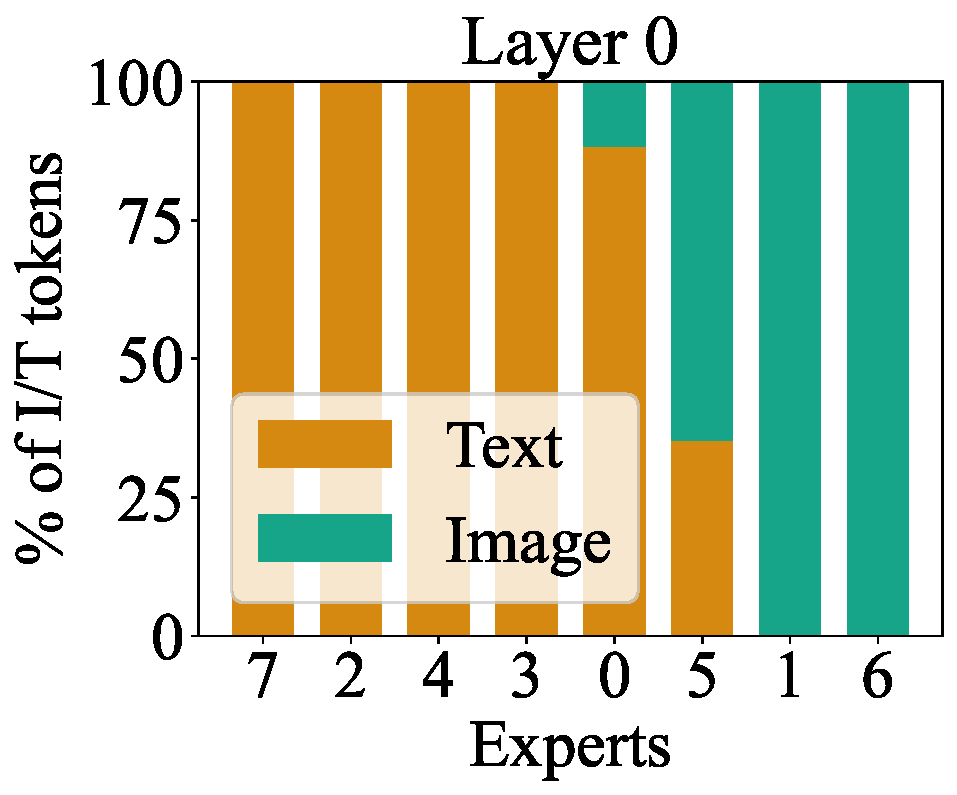
\includegraphics[height=0.27\textwidth]{assets/moes/specialization/sorted/tokens_assignment_obelics_1088_150_0.pdf}
    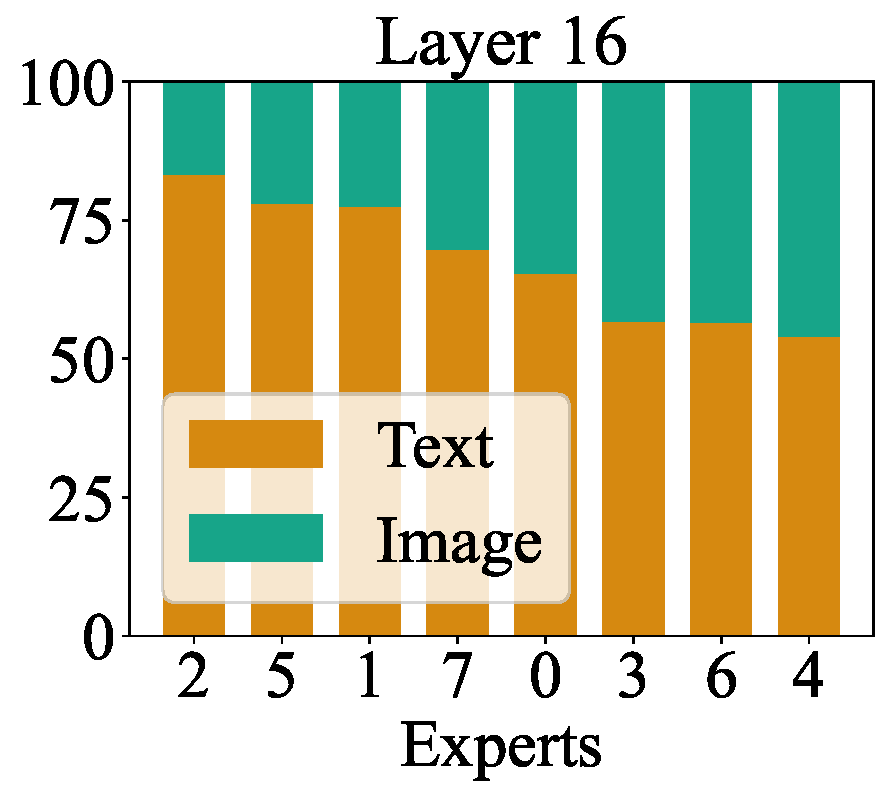
\includegraphics[height=0.27\textwidth]{assets/moes/specialization/sorted/tokens_assignment_obelics_1088_150_16.pdf}
    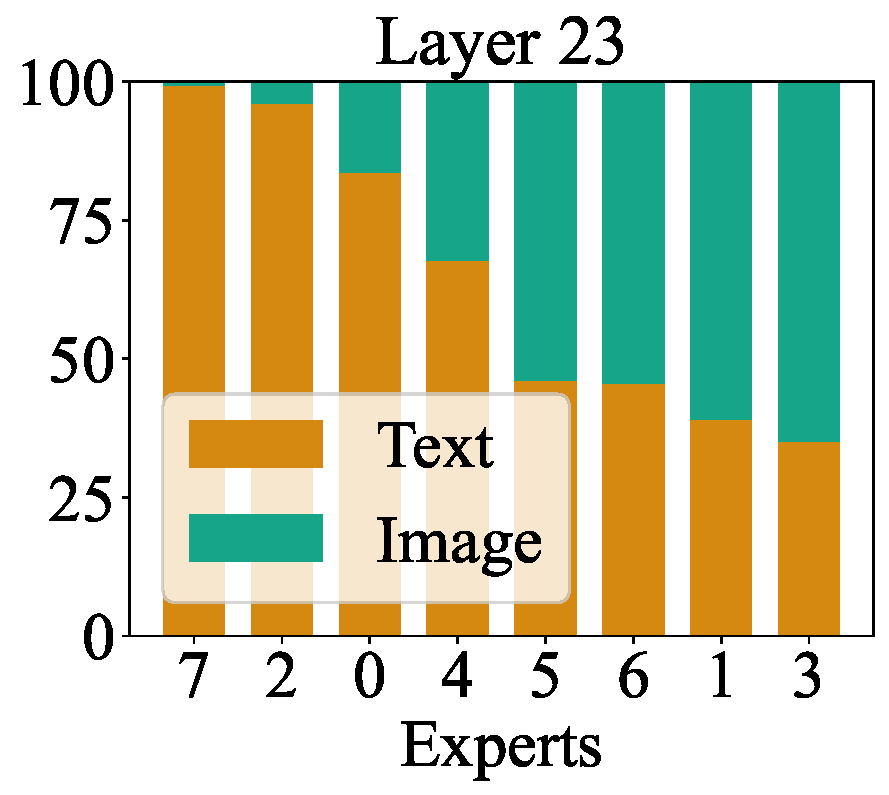
\includegraphics[height=0.27\textwidth]{assets/moes/specialization/sorted/tokens_assignment_obelics_1088_150_23.pdf}
    \end{subfigure}    \caption{\textbf{MoE 特化频率。} 从 Obelics 的交错数据中,路由到每个专家的文本和图像词元的百分比。专家按顺序排列以获得更好的可视化效果。第一层显示了最多的单峰值专家。}
    \label{fig:tokens_assignment}
\end{figure}

